\documentclass[italian]{memoir}
\usepackage{lmodern}
\usepackage[utf8]{inputenc}
\usepackage[italian]{babel}
\usepackage[T1]{fontenc}
\usepackage{float}
\usepackage{amsmath}
\usepackage{graphicx}
\usepackage{hyperref}

\usepackage{minted}
\usepackage{xcolor}
\usepackage{color}

%\usepackage[toc,page]{appendix}
\usepackage{titlesec}

\graphicspath{{./draws/}}

%\title{How to write a Report\\ for the Project of Distributed Systems}
\title{Progetto di Sistemi Distribuiti}

\author{Dott. Borsoi Diego\\Dott. Callegari Filippo\\ DMIF, University of Udine,
	   Italy\\(also the authors are distributed)}

\date{Version $\frac{1}{4}$, \today}

\begin{document}

\pagenumbering{gobble}
\maketitle
\newpage

\pagenumbering{alph}
\tableofcontents
\newpage

%%%%%%%%%%%%%%%%%%%%%%%%%%%%%%%%%%%
%			prefazione    		%
%%%%%%%%%%%%%%%%%%%%%%%%%%%%%%%%%%%
\pagenumbering{arabic}


\chapter{Introduzione}\label{ch:intro}

Il progetto in questione riguarda la creazione di un sistema distribuito per la comunicazione
	   fra dispositivi all'interno di una rete sparsa, tramite l'utilizzo di eventi.

\section{Descrizione del problema}

Ogni dispositivo corrisponde ad un nodo della rete ed è caratterizzato da:
\begin{itemize}
\item \textbf{Id} : numero univoco del nodo.
\item \textbf{Stato} : tupla di variabili che rappresentano delle specifiche caratteristiche
	   del nodo (es. temperatura di un sensore, stato di accensione di una termocoppia,
	   ecc).
\item \textbf{Regole} : insieme di regole del tipo ECA (Event Condition Action) che
	   possono attivarsi a seguito di un evento inviato al nodo. Queste regole possono
	   essere
	   di due tipi: locali, l'azione modifica solamente lo stato del nodo in cui si
	   attiva,
	   oppure globale, l'azione viene inviata a tutti i nodi della rete perché venga
	   letta
	   ed, in caso la valutazione della guardia associata sia positiva, eseguita.
\center$\{event;~condition;~action~|~\text{if}~guard~\text{then}~action\}$
\end{itemize}

Lo stato della rete si evolverà ogni qual volta un evento verrà attivato, andando
	   a sua volta ad innescare eventuali nuovi eventi e creando quindi una sequenza
	   di
	   azioni a cascata.

\section{Struttura dell'implementazione}

La rete in questione ha una struttura a mesh sparsa (cioè ogni nodo sarà al più
	   connesso a un numero di nodi molto basso, rispetto alla totalità).
I nodi sono idempotenti in modo tale da avere un sistema fortemente decentralizzato.
Le varie comunicazioni fra i nodi sono eseguite al di sopra di connessioni TCP, in
	   tal modo possiamo garantire la consegna di ogni messaggio nell'ordine prestabilito.
Per quanto concerne invece le comunicazioni riguardanti il sistema di $heartbeat$
	   (\ref{heartbeat}), queste vengono eseguite utilizzando connessioni UDP.

\section{Trasparenze}\label{Trasparenze}

Di seguito sono descritte le trasparenze che concergono e sono implementate dal sistema:

\begin{description} 
\item[Trasparenza ai fallimenti:] nel momento in cui un nodo fallisce/si disconnette,
	   il resto della rete continua a funzionare normalmente.
\item[Trasparenza alla scalabilità:] la rete può espandersi in dimensione senza
	   che il funzionamento dei nodi vari.
\item[Trasparenza alla mobilità:] un nodo può spostarsi all'interno della rete
	   senza che il funzionameto suo e degli altri nodi vada a modificarsi.
\end{description}

\section{Algoritmi}

Il sistema implementa solamente due algoritmi:
\begin{itemize}
\item \textbf{Flooding Algorithm:} viene usato inizialmente per la comunicazione di un'azione
	   a tutta la rete nel momento in cui in un nodo una regola globale o di transazione viene attivata.
\item \textbf{Lamport clock (modificato):} viene utilizzata una versione modificata
	   del Lamport clock per identificare i vari $flood$ eseguiti; questo clock viene
	   incrementato
	   solamente dall'invio (o ricezione) di un messasggio, e non dalle azioni interne
	   ad un nodo;
\item \textbf{Distributed Spanning Tree:} viene usato per ridurre il traffico di rete 
       quando la rete si è ``stabilizzata". Questo algoritmo mira a creare un albero di
       copertura nella rete.
\end{itemize}

Il sistema non implementa particolari algoritmi essendo che si vuole realizzare una
	   rete distribuita dove ogni nodo conosce esclusivamente i vicini ed evolve il
	   suo
	   stato solamente a causa di eventi ricevuti tramite dei messaggi.

\section{Testing}

Per testare il sistema verrà utilizzata un'entità $Ambiente$, la quale simulerà:
	   
\begin{itemize}
\item la creazione iniziale della rete, caricando da dei file appositi la struttura
	   degli stati, la lista di regole e la conformazione della rete
\item la scoperta di nuove connessioni
\item variazioni di variabili legate all'ambiente (es. temperatura registrata da
	   un sensore)
\item fallimenti di nodi
\item ritardi nell'invio di messaggi fra nodi
\end{itemize}

Ogni modulo verrà testato singolarmente ed infine verranno eseguiti dei test completi
	   del sistema.

\section{Piano di sviluppo}

Le future fasi di sviluppo seguiranno il seguente ordine:
\begin{enumerate}
\item Riunione con il committente per convalidare la risoluzione del problema
\item Implementazione ambiente virtuale per la gestione dei nodi 
\item Implementazione della struttura del nodo
\item Implementazione sistema $heartbeat$
\item Implementazione del sistema algoritmico
\item Test totale
\item Validazione
\end{enumerate}


%\section{Istruzioni}
%In this chapter you describe the main problem, and an idea of the solution.
%It is not necessary to be very detailed or formal, but it is important to explain
%	   which are the main aims and issues from the point of view of Distributed Systems:
%\begin{itemize}
%\item A description of the application.
%\item The overall structure of the implementation: how resources are deployed, which
%	   are the players, the r\^oles.
%\item The distributed system features (and the transparencies) and algorithms you
%	   intend to implement.
%\item Your plan for testing the system.
%\item A schedule for how you plan to carry out your design and implementation
%\end{itemize}

\chapter{Analisi}\label{ch:analisi}

In questo capitolo vengono descritti nel dettaglio requisiti funzionali e non funzionali
	   della soluzione proposta.

\section{Requisiti Funzionali}\label{sec:funcReq}

I requisiti funzionali individuati sono:
\begin{itemize}
\item \textbf{Categorizzazione di un nodo:} ogni nodo ha un tipo il quale ne identifica
	   lo stato e le sue regole;
\item \textbf{Modifica delle regole di un nodo:} ogni tipo di nodo può avere le
	   sue regole, codificabili attraverso la programmazione dello stesso;
\item \textbf{Modifica dello stato di un nodo:} ogni evento permette di avere o degli
	   \textit{effetti locali}, degli \textit{effetti globali} o degli \textit{effetti transizionali}:
	\begin{itemize}
	\item \textit{\textbf{effetti locali}}: la regola va a modificare lo stato interno;
	\item \textit{\textbf{effetti globali}}: la regola può modificare lo stato delle
	   variabili interne, e può generare un evento sugli altri nodi;
	\item \textit{\textbf{effetti transizionali}}: regola simile a quelle globali, ma con la differenza
	   che l'esecuzione avverrà in tutti i nodi coinvolti ``contemporaneamente";
	\end{itemize}
\item \textbf{Aggiunta dinamica di un nodo:} un nodo può essere aggiunto alla rete
	   in qualsiasi momento senza perturbarne la dinamicità, limitando l'aggiornamento
	   ai vicini a cui si collega.
\item \textbf{Esecuzione di un'azione ricevuta dai vicini:} nel momento in cui un
	   nodo riceve un messaggio dai propri vicini esso va a verificare la soddisfacibilità
	   della guardia (se presente) e nel caso di una valutazione positiva viene eseguita
	   l'azione associata, andando quindi a modificare il proprio stato.
\item \textbf{Attivazione di una regola:} ogni qual volta avviene un cambiamento
	   nello stato di un nodo, viene eseguito un controllo delle regole, per vedere
	   se gli
	   eventi generati possano attivare una o più regole del nodo; nel caso in cui
	   una regola venga attivata, in base al tipo (locale, globale o transazione) viene portata a termine
	   l'azione corrispondente.
\end{itemize}

\section{Requisiti Non Funzionali}

I requisiti non funzionali individuati sono:
\begin{itemize}
\item \textbf{Decentralizzazione:} nessun nodo ha il controllo dell'ordine degli
	   eventi, grazie al fatto che ogni nodo è idempotente;
\item \textbf{Tolleranza ai guasti:} poiché tutti i nodi sono idempotenti, nel momento
	   in cui un nodo si scollega dalla rete, la rete rimanente continua ad operare
	   normalmente;
\item \textbf{Etereogenità:} fintanto che i nodi aggiunti utilizzano il protocollo
	   descritto, qualunque nodo di qualunque tipo (hardware o categoria) potrà essere
	   aggiunto alla rete;
\item \textbf{Scalabilità:} l'aggiunta dinamica dei nodi alla rete permette di scalare
	   orizzontalmente con estrema facilità;
\item \textbf{Trasparenze:} le trasparenze implementate sono quelle descritte al
	   capitolo precedente (paragrafo \ref{Trasparenze}).
\end{itemize}

%\chapter{Analysis}\label{ch:analysis}
%
%In this chapter, we describe in detail functional and non-functional requirements
%	   of a solution for the problem.
%
%\section{Functional requirements}
%Which functions must be offered to users / other programs?  Which are the input
%	   data and the output data? Which is the expected effect? 
%
%\section{Non functional requirements}
%Everything about mode and transparencies: availability, mobility, security, fault
%	   tolerance, etc.
%
%Are there execution time bounds? Minimum data rates?
%
%If requested, specific platforms/languages/middlewares requirements for the implementation
%	   can be decided here. (E.g.: if the project is on a SOA, we may request that
%	   functions
%	   are offered via SOAP or RESTful services). 



\chapter{Progetto}\label{ch:progetto}

In questo capitolo vengono descritti in modo più approfondito l'achitettura del
	   progetto, i moduli, i protocolli e gli algoritmi utilizzati.

\section{Architettura logica}

Essendo tutti i nodi costruiti al medesimo modo, di seguito presentiamo la struttura
	   di uno singolo di essi. 

\begin{figure}[H]
\makebox[\linewidth][c]{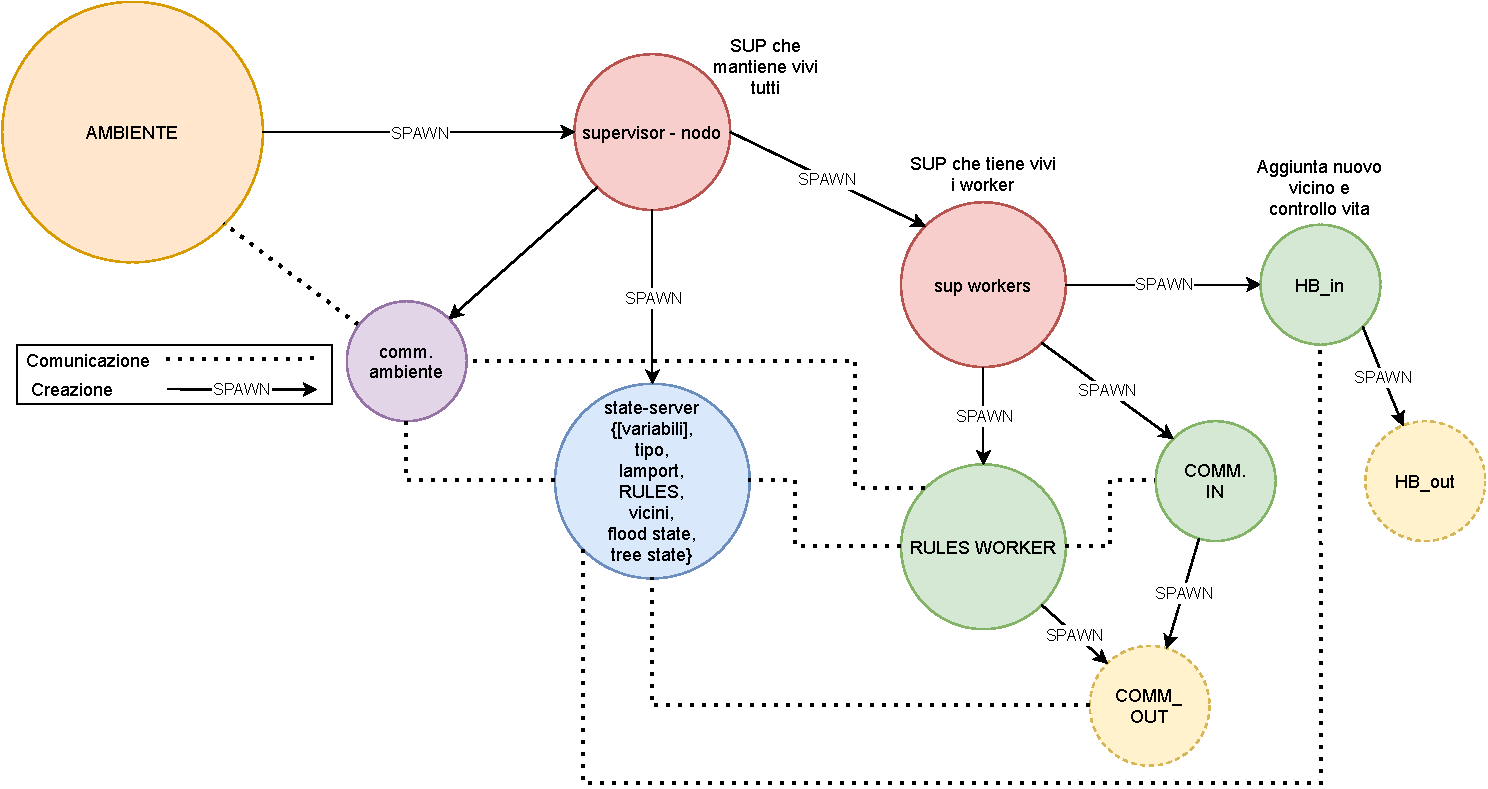
\includegraphics[scale=0.65]{draw_nodeworker.pdf}}
%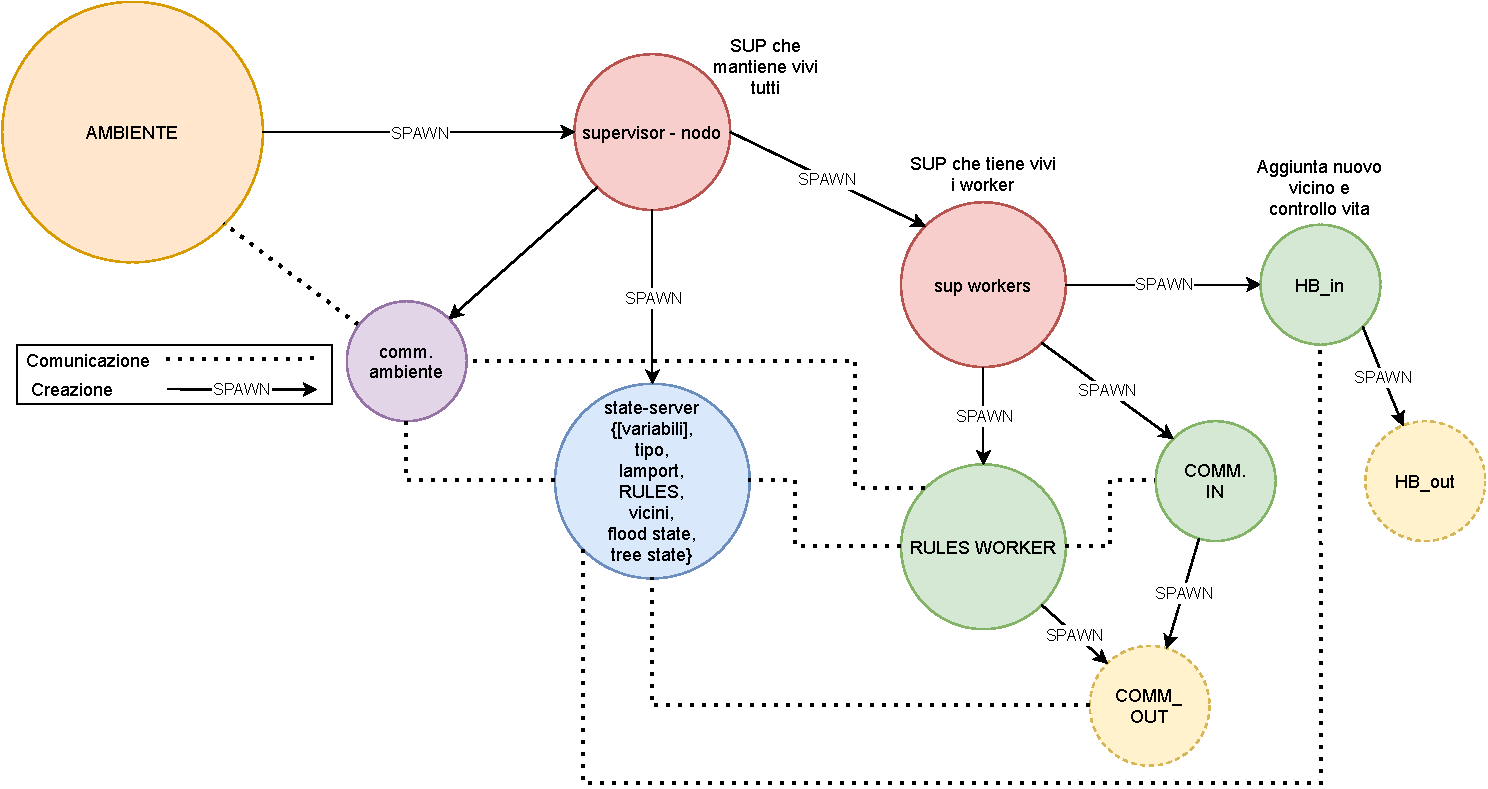
\includegraphics[scale=0.6]{draw_nodeworker.pdf}
%\centering
\caption{Struttura gerarchica dei moduli di un nodo e visualizzazione delle connessioni
	   fra di essi.}
\label{img:struttura_nodo}
\end{figure}

Come si può vedere dalla figura \ref{img:struttura_nodo}, ogni nodo è formato dai
	   seguenti moduli:
\begin{itemize}
	\item \textbf{Supervisor nodo:} modulo che cerca di manterene sempre operativi gli
	   altri moduli interni. Se questo componente si riavvia equivarrebbe ad un riavvio
	   del nodo, e quindi la conseguente perdita della modifica agli stati interni.
	   I moduli
	   da lui controllati sono:
	\begin{itemize}
	\item \textbf{State server:} questo modulo manterrà tutte le variabili locali al
	   nodo, che verranno modificate durante l'operatività dello stesso. Queste variabili
	   sono:
		\begin{itemize}
		\item stato del nodo;
		\item lista delle regole associate al nodo;
		\item tipo del nodo;
		\item stato delle waves; %sia clock che cose precedenti
		\item informazioni sui nodi vicini;
		\item id univoco del nodo;
		\end{itemize}
	\item \textbf{Supervisor dei workers:} modulo che si occupa di gestire i moduli
	   a lui dipendenti, riavviandoli in caso di ``crash". Questi sono:
		\begin{itemize}
		\item \textbf{heartbeat sense:} si occupa di controllare la ``vitalità" dei vicini,
	     di istanziare le connessioni con essi e di mantenere la ``spanning tree" della rete.
	     Ogni qual volta che deve comunicare con dei vicini affini, creerà un processo effimero
	     (HB\_out);
		\item \textbf{communication in:} si occupa di gestire tutti i messaggi in ingresso
	   relativi al nodo in questione;
		\item \textbf{rules worker:} si occupa di applicare le azioni ricevute dai nodi
	   vicini ed eventualmente eseguire una delle regole a lui locali al momento dell'attivazione;
	   lui si occuperà anche di propagare le regole che generano degli eventi verso
	   gli
	   altri nodi, interpellando il modulo ``\textit{communication out}'' 
	  (modulo apposito per l'invio dei messaggi ai nodi vicini).
		\end{itemize}
	\end{itemize}
\end{itemize}

Come è stato accennato in precedenza verrà sviluppato un ulteriore modulo chiamato
``\textbf{\textit{Ambiente}}": questo modulo permette di simulare le interazioni
	   che avverrebbero nel mondo reale. Nel dettaglio, le funzionalità del modulo
	   sono:
\begin{itemize}
	\item il "discovery" dei vicini;
	\item cambiamento delle variabili non dipendenti dalle regole (temperatura dell'ambiente/GPS/...);
	\item simulazioni di disservizi di rete;
	\item simulazione di guasti (temporanei o non) di un nodo;
	\item topologia della rete.
\end{itemize}
Dal punto di vista del nodo ci troviamo quindi costretti ad aggiungere un ulteriore
	   modulo fittizio (\textbf{\textit{comunicazione ambiente}}) per permettere la
	   comunicazione
	   con l'ambiente.

\section{Protocolli ed algoritmi}

Di seguito verranno descriti nel dettaglio i vari protocolli ed algoritmi utilizzati.

\subsection{Controllo e attivazione delle regole}

Nel momento in cui il sistema riceve un'azione da eseguire (dopo aver controllato la validità e che appartenga ad una wave non ancora ricevuta) si innesca la seguente serie di azioni:
\begin{enumerate}
\item il modulo \textit{communication IN} invia l'azione da eseguire al modulo \textit{rules worker};
\item quest'ultimo utilizza una funzione dello \textit{state server} per modificare lo stato del nodo in accordo all'azione ricevuta;
\item il \textit{rules worker} esegue quindi un controllo sulle regole andando ad identificare quali possono essere attivate dalla modifica appena eseguita;
\item per ciascuna regola che viene attivata viene testata la condizione e in caso di risultato positivo:
\begin{itemize}
\item se la regola è del tipo \textit{locale}, viene eseguita l'azione associata
\item se invece la regola è del tipo \textit{globale}, viene eseguita l'azione associata (in caso di guardia con valutazione positiva) e viene passata ad un processo di \textit{communication OUT}, istanziato appositamente, che genera una nuova wave di messaggi inviando ai vicini la nuova azione.
\end{itemize}
\end{enumerate}

\subsection{Heartbeat}\label{heartbeat}
Il protocollo di ``heartbeat'' serve per mantenere consistente lo stato dei vicini
	   di un nodo. Questo infatti controlla la loro vitalità e sarà componente chiave
	   per l'aggiunta di un nuovo nodo.

L'algoritmo si suddivide quindi in tre componenti:
\begin{itemize}
	\item \textit{ECHO}: similmente al protocollo ICMP, si fa una richiesta di echo
	   al vicino. Se questa ``\textit{ECHO\_RQS}" andrà a buon fine, il primo nodo che
	   istanzia una richiesta di ``\textit{ECHO}" richeverà un pacchetto di ``\textit{ECHO\_RPL}".
	   Definiamo come $\tau$ il tempo che intercorre tra un messaggio di \textit{ECHO} ed
	   un'altro. Se un nodo non rispondesse entro $2\tau$ ad una \textit{ECHO\_RQS}, questo
	   verrà considerato come non più collegato. Ogni \textit{ECHO\_RPL} conterrà il clock
	   attuale del vicino.
	\item \textit{ADD\_NEW\_ND}: similmente al protocollo DHCP, nella fase di aggiunta
	   di un nodo alla rete, il nuovo nodo si annuncia al suo vicino ``fisico'', chiedendo
	   le informazioni essenziali per poter partecipare attivamente alla rete. Questo sarà
	   spiegato più in dettaglio nella prossima sezione.
	\item \textit{TREE\_STATE}: questa componente si focalizza sulla gestione dell'albero di copertura della rete.
	Sarà analizzato in dettaglio nei paragrafi successivi.
\end{itemize}

\begin{figure}[H]
\centering
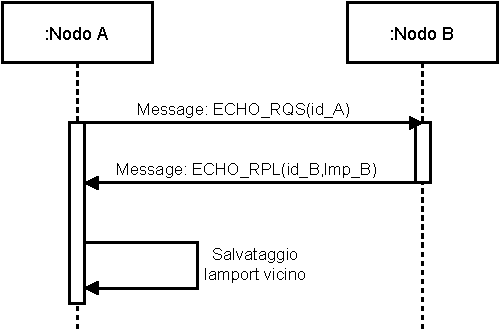
\includegraphics{HeartbeatDiagram.pdf}
\caption{Sequence diagram dei messagi usati per il sistema di \textit{heartbeat}.}
\label{img:heartbeat}
\end{figure}

\subsection{Aggiunta di un nuovo nodo}
L'aggiunta di un nodo è una parte complicata del sistema: bisogna tener conto della
	   possibilità che la rete si partizioni. Questo si può verificare nel caso in cui
	   un nodo si riavvii. Il partizionamento della rete è visto come caso particolare
	   di aggiunta di un nodo alla rete.

L'aggiunta di un nuovo nodo si compone dei seguenti passi:
\begin{enumerate}
	\item \textit{ADD\_NEW\_ND}: il nuovo nodo manda la richiesta di aggiunta alla rete
	   a tutti i suoi vicini inviando il proprio id;
	\item \textit{ADD\_NEW\_NB}: il nodo che deve aggiungere il nuovo nodo risponde
	   con un messaggio contenente $(clock,id)$.
\end{enumerate}
A questo punto, una volta che per ogni vicino ho i suoi parametri di clock, i casi
	   possibili sono 2:
\begin{enumerate}
	\item \textbf{tutti i nodi hanno medesimo clock:} imposto il mio clock al clock
	   comune;
	\item \textbf{esiste un clock massimo:} imposto il mio clock al valore massimo,
	   e rispondo con \textit{UPD\_LMP} a tutti i miei vicini che non hanno il clock al
	   massimo. Questi a loro volta manderanno a tutti i loro vicini, con clock diverso
	   da quello scelto, il nuovo valore.
\end{enumerate}

\begin{figure}[H]
\makebox[\linewidth][c]{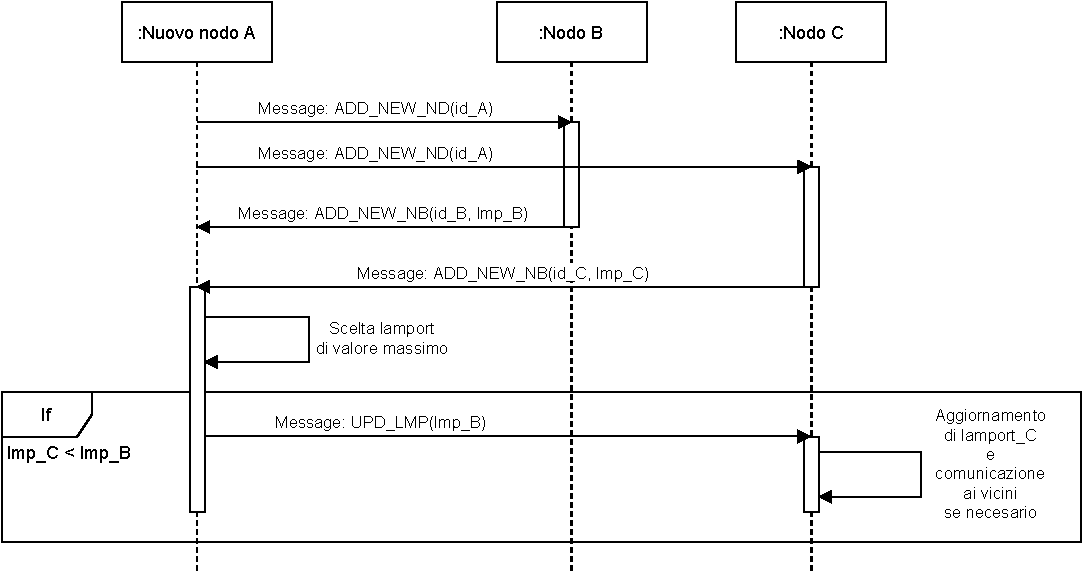
\includegraphics[scale=0.9]{NewNodeDiagram.pdf}}
\caption{Sequence diagram dei messagi usati per laggiunta di un nuovo nodo alla rete.}
\label{img:newnode}
\end{figure}

\subsection{Two-phases Rules (Transazioni)}
Questo è un protocollo definito come ``two-phases commit", ovvero permette l'esecuzione in
contemporanea su più parti di almeno un'azione. Questo protocollo è stato modificato rispetto
l'originale, in quanto, non avendo l'obbligo di avere sempre uno stato consistente tra i nodi,
ci permette di semplificarlo. Le fasi sono quindi le seguenti:
\begin{enumerate}
    \item \textit{discovery}: troviamo tutti i nodi nella rete che sono interessati ad eseguire la
    transazione. Il nodo inizializzatore manda nella rete un messaggio di richiesta di transazione,
    il quale contiene delle condizioni per partecipare. Se un nodo è interessato, risponderà all'inizializzatore
    dicendogli di essere interessato.
    \item \textit{start}: il nodo inizializzatore darà inizio alla transazione per i nodi interessati.
\end{enumerate}
All'interno di questo protocollo, come possiamo vedere nell'immagine \ref{img:transazioni}, vengono tenuti dei timeout
di controllo, al fine di non rimanere bloccato nello stato di transizione: se un nodo decide di partecipare 
alla transazione, allora non potrà eseguire altre regole.

\begin{figure}[H]
\makebox[\linewidth][c]{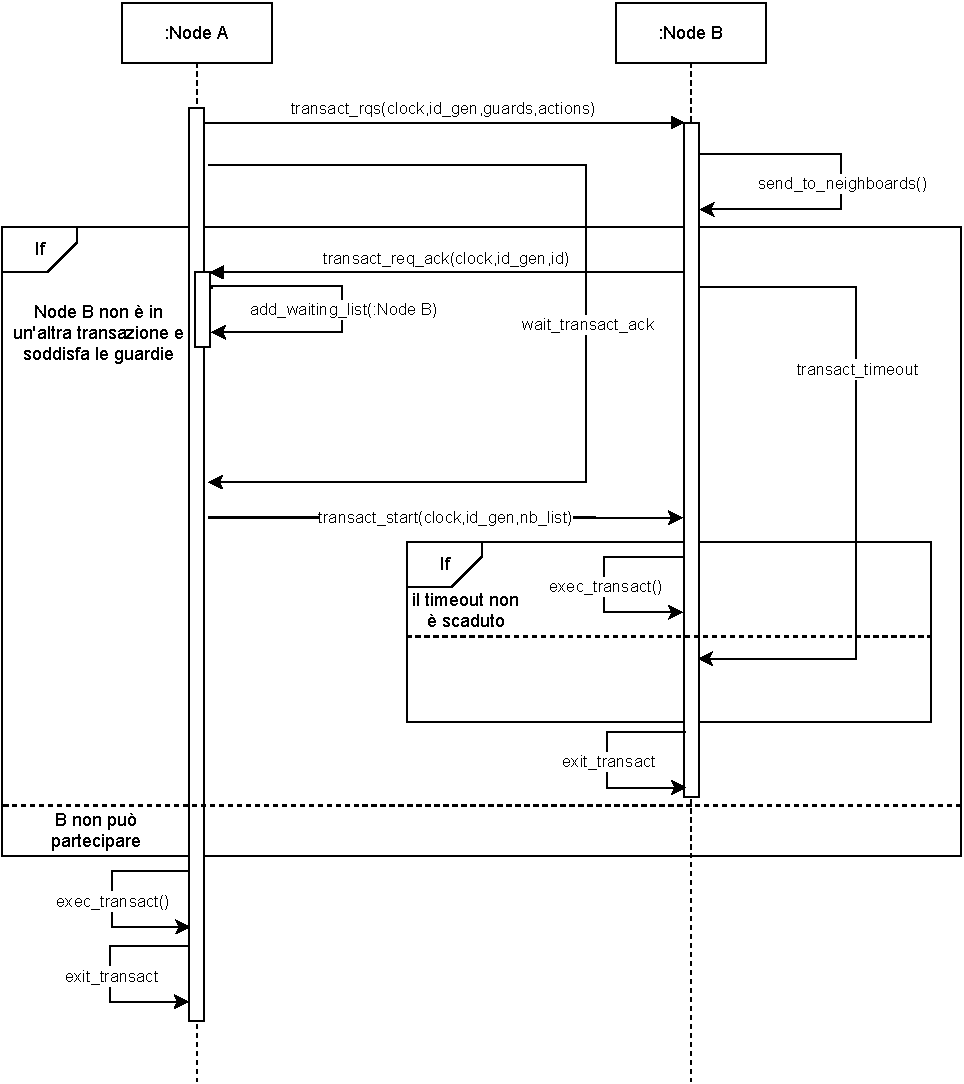
\includegraphics[scale=0.9]{Transaction_diagram.pdf}}
\caption{Sequence diagram del protocollo adottato per le regole di transaction.}
\label{img:transazioni}
\end{figure}

\subsection{Algoritmo: Flooding}
Ogni qual volta si crea una regola che genera un evento "globale", ogni nodo spedirà
	   ai suoi vicini un messaggio contenenta un'azione da eseguire. Questi, una volta ricevuto,
	   aggiorneranno il loro "wave count" (tenuto dal clock, spiegato successivamente),
	   e passerà all'esecuzione dell'istruzione condizionata contenuto nel messaggio. Al
	   fine di evitar la presenza di messaggi vecchi nella rete, ogni messaggio conterrà
	   la coppia $(clock,id\_gen)$: questo verrà salvato localmente nel nodo ricevente,
	   e verrà mantenuto in memoria al fine di verificare se un messaggio ricevuto non
	   è già stato eseguito. Ogni nodo quindi spedirà una copia del messaggio a tutti
	   i suoi vicini (a patto non l'abbia già ricevuto in passato), meno a quello da cui
	   l'ha ricevuto. Queste strategie applicate faranno si che i messaggi circolanti nella
	   rete siano il minor numero possibile, e nell'eventuale creazioni di cicli nella rete,
	   dovuta alla topologia della stessa, siano soppressi alla prima occasione utile.

\begin{figure}[H]
\makebox[\linewidth][c]{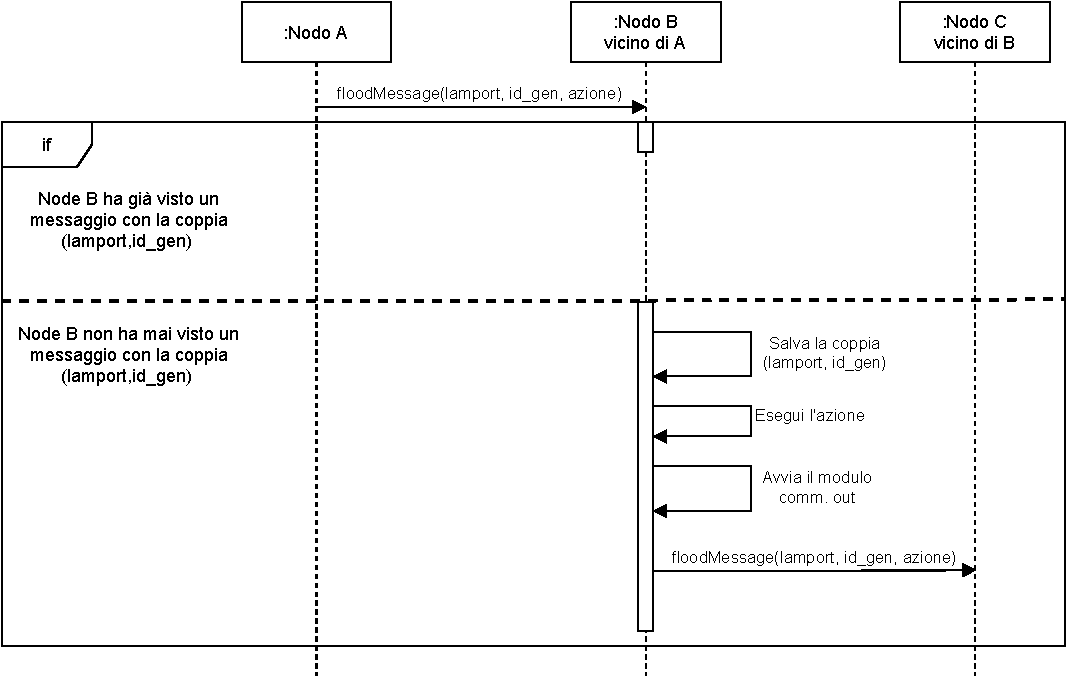
\includegraphics[scale=0.8]{FloodDiagram.pdf}}
\caption{Sequence diagram dei messaggi usati per l'algoritmo di flooding.}
\label{img:flooding}
\end{figure}

\subsection{Algoritmo: Lamport modificato}
Il ``Clock di Lamport" ci permette di dare una certa conseguenza temporale alle azioni.
	   Questo sarà un numero intero crescente, ed identificherà ogni wave generata. Alla
	   generazione di una wave ogni nodo userà il suo clock interno, incrementato, per
	   identificarla. Questo ci permette, come già abbiamo spiegato, di controllare la
	   propagazione dei messaggi. Sia quindi $Lmp_i$ il clock della nuova wave ricevuta
	   e $Lmp_n$ il clock del nodo corrente. Le azioni intraprendibili sono:
\begin{itemize}
	\item $Lmp_i = Lmp_n + 1$: eseguo immediatamente l'azione in essa contenuta ed aggiorno
	   il valore di $Lmp_n$;
	\item $Lmp_i > Lmp_n + 1$: aspetto un preimpostato timeout (es: $5\tau$) prima di
	   eseguire l'azione di $Lmp_i$, in modo tale da poter ricevere le wave mancanti, e
	   quindi mantenere l'ordine causale delle azioni;
	\item $Lmp_i < Lmp_n$: vado ad eseguire l'azione solo nel caso in cui tutte le variabili
	   coinvolte non siano già state modificate da una wave ad essa successiva, cioè con
	   $clock > Lmp_i$.
\end{itemize}

\subsection{Algoritmo: Distribuited Spanning Tree}\label{algo:dstp}
L'albero di copertura (o spanning tree) è un protocolo distribuito tra i nodi ideato per limitare il numero di messaggi nella rete. Questo protocollo risulta essere una versione modificate el più noto \textit{STB} (IEEE 802.1aq). Tutto questo protocollo viene eseguito sempre dal sistema di heartbeat, in quanto strettamente correlati.

Questo protocollo si divide in 3 fasi:
\begin{itemize}
    \item \textit{\textbf{discovery}}: in questa fase, il nodo che si sta connettendo esplora la rete, e dice a tutti di essere la radice. A seconda delle condizioni, esplicitate in dettagli nel capitolo successivo, potrà effettivamente esserlo o meno;
    \item \textit{\textbf{listening}}: in questa fase, l'albero risulta stabile. Ogni $\bar{\tau}$ la radice ``eletta" manda dei pacchetti di keep alive ai figli. Nel momento in cui un la radice cesserà la sua permanenza nella rete, si passerà alla fase successiva;
    \item \textit{\textbf{transiction}}: in questa fase, per almeno uno componente della rete, la radice risulta non più raggiungibile. In questa fase i nodi coinvolti, non possono accettare la vecchia radice. Questa fase avviene quando un nodo perde la sua ``radice", o quando lo spanning tree perde la radice che lo genera.
\end{itemize}

La scelta della radice avviene in maniera deterministica, sfruttando l'identificatore univoco di cui ogni nodo è dotato. Definiamo $<saved\_root, saved\_len, saved\_nh>$ la tupla che identifica i dati di radice attualmente salvata, la mia attuale distanza e attraverso quale vicino riesco a raggiungerla, mentre definiamo come $<root, len, nh>$ la tupla proposta dai miei vicini. A questo punto la scelta per un nodo della sua radice avviene come segue:
\begin{itemize}
    \item $saved\_root > root$: la radice proposta è inferiore alla mia e sarà scelta come mia nuova radice;
    \item $saved\_root = root \land saved\_len + 1 < len$: il mio vicino è ha una distanza peggiore della mia, lo avviso che il mio percorso potrebbe essere migliore;
    \item $saved\_root = root \land saved\_len > len + 1 $: la mia distanza è peggiore di quella proposta, mi sposto sul mio vicino, in maniera di esser più vicino alla radice;
    \item $saved\_root = root \land saved\_len = len + 1  \land nh\_saved > nh$: per questioni di determinismo, se la distanza e la radice proposta sono identiche, scelgo come ``porta" verso la radice il mio vicino con id minore degli altri.
\end{itemize}

A questo punto possiamo scegliere anche a quali dei nostri possiamo inviare i messaggi: poichè ogni nodo è informato se è un nodo scelto o meno, se inoltriamo i messaggi solo ai vicini in cui sono stato scelto o al vicino che io ho scelto, posso raggiungere tutta la rete con un numero minimo di messaggi. A tal fine ogni vicino potrà assumere 3 vari stati:
\begin{itemize}
    \item\textit{root\_port}: vicino scelto per raggiungere la radice;
    \item\textit{active}: vicino che mi ha scelto per raggiungere la radice;
    \item\textit{disabled}: vicino che non dipende da me.
\end{itemize}


\section{Architettura fisica e deployment}
Per quanto riguarda l'architettura fisica è necessario l'utilizzo di microcalcolatori,
	   come dei ``Raspberry" o degli ``Arduino". Ogni nodo corrisponderebbe fisicamente
	   ad una di queste schede, avendo quindi la possibilità d'utilizzare più nodi
	   per
	   il medesimo ``apparato".

Non è strettamente necessario l'ausilio di microcalcolatori: potrei concentrare
	   all'interno di un singolo calcolatore più nodi, a patto che siano gestiti in
	   maniera
	   consona. 

Come descritto in precedenza, questi comunicherebbero con protocollo TCP ed UDP,
	   non interessandoci quindi di tutta la rete sottostante.

Visto l'esempio a cui abbiamo pensato, si ritiene ideale l'utilizzo di connessioni
	   wireless.
\section{Piano di sviluppo}
Le \textbf{funzionalità di base} che verranno implementate sono:
\begin{itemize}
	\item comunicazione tra nodi;
	\item sistema di flooding;
	\item sistema di heartbeat;
	\item gestione dell'aggiunta di un nodo alla rete;
	\item gestione del riavvio di un nodo nella rete;
	\item impostazione iniziale dei nodi (ambiente);
	\item programmazione dei nodi;
	\item sistema basico d'esecuzione delle regole.
\end{itemize}
Sono state inoltre individuate le seguenti \textbf{funzionalità avanzate}:
\begin{itemize}
	\item sistema avanzato d'esecuzione delle regole;
	\item salvataggio dello stato del nodo su files interni al controllore;
	\item riprogrammazione dinamica del nodo;
	\item implementazione di un \emph{calculus} locale.
\end{itemize}

\chapter{Implementazione}
In questo capitolo tratteremo le scelte implementative avvenute nel corso del progetto. ci focalizzaremo man mano nei vari dettagli, cercando di spiegarne le motivazioni delle varianti adottate dai vari algoritmi o protocolli standard.

\section{Software e hardware}
Per l'implementazione non si è seguita una vera e propria scelta hardware, ma si è tenuto conto i vincoli, quali scarsa capacità computazionale e scarsa memoria.

A livello software la scelta è ricaduta su Erlang, in quanto linguaggio fortemente orientato ai threads, funzionale e con spiccata capacità alle connessioni. Altra peculiarità sono le librerie messe a disposizione dallo stesso tramite OTP (Open Telecom Platform). Di queste librerie sfrutteremo fortemente dei ``behavior module'', quali \textit{gen\_server} e \textit{supervisor}, i quali danno a disposizione l'astrazione del meccanismo del client/server e di supervisione dei threads del processo in vita. I moduli sviluppati più interessanti saranno quindi descritti in dettaglio nei paragrafi successivi.

\section{Utilizzo dei ``Supervisors"}
Come già accennato, il meccanismo dei supervisor permette di gestire tutti i threads che verranno creati per i vari processi del nodo. Come si può notare in figura \ref{img:struttura_nodo}, abbiamo due supervisor: uno per mantenere la vitalità di tutti i processi interni (dal modulo di ``state\_server" al più semplice ``HB\_out").

Il primo supervisor, generato dal modulo \textit{``supervisor\_nodo"}, provvede a sopperire alla necessità di mantenere in vita tutti quei dati essenziali al funzionamento del nodo. Al suo interno infatti verrà istanziata la tabella ``ets'' dove vengono salvate tutte le informazioni relative alle funzionalità del nodo (lo stato dell'albero, il clock, le regole,...), verrà istanziato il thread designato alla comunicazione con l'ambiente, e per finire anche il thread che si occuperà di manipolare in maniera \textit{sicura} i parametri del nodo. Ultimo, ma non per importanza, verrà generato come figlio del supervisor generale del nodo, il supervisor dei ``workers'', che si occuperà di mantenere in vita i thread per l'heartbeat e per chi interpreterà le regole.

Codice d'esempio si trova Nell'appendice \ref{code:supervisor}.

\section{Heartbeat (module: HB\_in)}\label{impl:hbin}
Come descritto precedentemente, nel modulo \textit{HB\_in} possiamo trovare tutti i meccanismi legati alla gestione della rete e delle sue funzionalità come tale. Nello specifico, questo si occupa solamente di controllare la ``vitalità" di un nodo e di creare un albero di copertura della rete stabile, con tutti i suoi protocolli annessi.

\subsection{Heartbeat - consistenza della rete}
La prima funzionalità (appunto, garantire la consistenza della rete), serve a garantire che se un nodo a me vicino si spenga o diventi non più raggiungibile, allora non devo più considerarlo come mio vicino. La consistenza della rete avviene tramite alcune variabili di stato interne al modulo, identificabili dalla tupla:
$$
    <neighb\_clocks, neighb\_state>
$$
Il primo valore della tupla identifica una mappa di tipo $<id,clock>$, e mi serve nel momento in cui ho un aggiornamento del clock interno dovuto al ricongiungimento di una rete partizionata: per cercar di garantire la consistenza delle wave di regole che si propagheranno nella rete, dovrò cercare di allineare tutti i componenti della rete al medesimo clock.
Il secondo valore della tupla identifica una mappa del tipo $<id,stato>$: per controllare la vitalità di un nodo devo infatti verificarne la sua presenza attraverso il meccanismo di ``echo" descritto nel paragrafo \ref{heartbeat}. Alla creazione del nodo suppongo che tutti i miei vicini siano ``vivi", e sono tali fino a prova contraria (ovvero quando non rispondono più agli echo). Gli \emph{stati} assumibili dai vicini in questa mappa quindi saranno:
$$
stato(\eta:neightboard)=\begin{cases}
                         alive, & \mbox{se }\eta\mbox{ ha risposto all'ultimo echo} \\
                         maybe\_death, & \mbox{se }\eta\mbox{ non ha risposto all'ultimo echo}\\
                         death, & \mbox{se }\eta\mbox{ non ha risposto agli ultimi due echo}
                   \end{cases}
$$
con $\eta$ vicino di ogni nodo.\\
Si rimanda all'appendice \ref{code:heartbeat} per ulteriori esemplificazioni.

Un vicino si dichiara $maybe\_death$ dopo $\tau = 5s$, e $death$ dopo $2*\tau$.

\subsection{Heartbeat - spanning tree}
Come abbiamo già accennato in precedenza, il protocollo di spanning tree prende spunto dal più famoso \textit{spanning tree protocol} adottato dai bridge. 

Questo protocollo basa il suo funzionamento sull'interscambio di tuple:
\begin{enumerate}
\item $<tree\_state,<root,len,nh>>$: questa tupla indica lo stato dell'albero per il nodo che la propaga. Essa infatti contiene chi è la radice per quel nodo, quanto essa è distante e chi è che manda fuori il pacchetto;
\item $<tree\_ack, id>$: questo pacchetto avvisa il nodo vicino che verrà usato per ``instradare" pacchetti nella rete;
\item $<tree\_rm\_rp, id>$; avvisa la mia vecchia \textit{root\_port} che non la utilizzo più per instradare pacchetti.
\end{enumerate}
Per ulteriori delucidazioni su come vengono instraprese le scelte si rimanda al paragrafo \ref{algo:dstp}.

La necessità di avvisare i nodi vicini che li usiamo come root port o meno nasce dalla particolare situazione in cui ci troviamo: poichè non abbiamo un vero e proprio ambiente dove nodo non designato al raggiungimento della radice comunica con tutti i nodi di quella zona, siamo costretti ad avvisare se un nodo è una root\_port o meno. Questo passaggio complica la rete, in quanto crea un ``overhead" di messaggi normalmente non contemplato dal protocollo originale.

Ulteriormente, poichè tutti i nodi non possono accorgersi in ``tempo reale" della situazione delle loro ``porte" (dato che sono tutte connessioni punto-punto), si richiede l'utilizzo ulteriori clock per la correttezza dell'albero dell'albero: uno sarà settato al controllo dell'effettiva vitalità di un vicino, uno per i timeout per la vitalità della radice, ed uno per non accettare l'id della vecchia radice come nuova radice. L'utilizzo di questi clock creano altri messaggi di saturazione della ``rete emulata", desincronizzano i vari nodi, e peggiorano le performance, imponendo necessariamente una potenza di calcolo più grande di quanto non sia una rete fisica.

Nel nostro specifico caso, viene fissato $\bar{\tau} = 2 s$, come timeout  $2*\bar{\tau}$, come timeout per accettare di nuovo la vecchia radice $3*\bar{\tau}$.

\subsection{Heartbeat - comunicazioni in uscita}
Per le comunicazioni in uscita, come possiamo notare da alcune linee di codice dell'appendice \ref{code:heartbeat}, interpelliamo il modulo \textit{HB\_out}: questo modulo gestisce le comunicazioni in uscita, compresi gli errori di comunicazione. Parametri richiesti per la comunicazione verso l'esterno sono:
\begin{itemize}
\item \textit{pacchetto}: il messaggio già confezionato da inviare
\item \textit{vicini}: una lista iterabile di vicini a cui mandarlo (per precisione, al loro hearbeart).
\end{itemize}
Questo thread viene direttamente creato dal modulo di \textit{HB\_in}, ed appena esaurisce la lista cessa la sua esistenza.

Si rimanda al file in \texttt{src/HB\_out.erl} per vedere in dettaglio il suo funzionamento.

\section{Memoria dei parametri (module: state\_server)}
Ogni nodo, come esplicitato nei requisiti funzionali (paragrado \ref{sec:funcReq}), necessita d'essere programmabile e d'avere un'insieme di variabili di stato proprie. Oltre a questo, abbiamo necessità di conoscere e di poter interpretare delle regole definite all'avvio del nodo. Inoltre, poichè abbiamo a che fare con un'ambiente virtualizzato, necessitiamo di sapere quali sono i vicini con cui collabora.

Tutte queste informazioni, come già esplicitato nel capitolo precedente e nei paragrafi precedenti, sono salvate all'interno di uno ``state server'', il quale opera su delle tabelle persistenti, fronteggiate dal supervisor del nodo, al fine di non aver problematiche in caso di fallimenti.

Lo state server è incentrato in un'ottica client/server: per questo motivo il suo behavior module è \textit{gen\_server}.

Lo state server si occupa quindi di accedere in maniera sicura e non concorrenziale alle variabili a suo carico, al fine di non generare situazioni di deadlock o starvation.

Lo stato dello \textit{state\_server} sarà quindi composto dalla tupla
$$
    <vars\_table, rules\_table, neighb\_table, node\_params\_table>
$$
dove ogni campo equivale a:
\begin{itemize}
    \item \textit{vars\_table}: tabella delle variabili;
    \item \textit{rules\_table}: tabella delle regole;
    \item \textit{nb\_table}: tabella dello stato dei vicini;
    \item \textit{node\_params\_table}: tabella dei parametri interni al nodo.
\end{itemize}

I valori associati alla terza componente sono strettamente correlati a quanto affrontato nel paragrafo \ref{impl:hbin}: al suo interno troveremo delle tuple con i valori legati allo spanning tree per cui sapremo se inoltrare o meno un messaggio a quel nodo. L'inoltro di un messaggio verso un nodo avviene solo nel caso in cui il vicino sia in stato $active$ o $root\_port$.

I valori associati alla quarto membro della tupla sono invece legati ad informazioni chiave per identificare il nodo di appartenenza. Al suo interno possiamo trovare alcune voci, quali, ad esempio, il suo identificativo univoco, che tipo di nodo è per la rete, quante \textit{``rules wave"} ha visto, il suo clock interno e chi è la sua radice. Queste informazioni sono identificative ed univoche per un nodo, e sono il suo stato interno.

Il significato puntuale della prima e della seconda componente questa tupla verranno affrontati in miglior dettaglio nel paragrafo \ref{impl:rules_worker}. 

Poichè lo state server è l'unico a poter manipolare le variabili del nodo, al suo interno avrà un piccolo ``interprete" per manipolare e controllare le variabili. Questo avviene in maniera ricorsiva mediante l'utilizzo di una funzione ricorsiva chiamata ``check\_condition" (si rimanda all'appendice \ref{code:stateserver} per ulteriori delucidazioni).

\section{Esecutore dei comandi (module: rules\_worker)}\label{impl:rules_worker}

blablablablablabla\\
step per il parsing delle regole blablablabla

\subsection{propagazione delle regole}
blablablabla\\
mi piace che vada fuori tutto subito e poi vedo se posso fare qualcosa\\
blablablablabla

\subsection{Organizzazione delle regole}
effetti locali/glob/trans\\
blablablablabl\\
struttura in appendice\ref{code:rulesstruct}%importa o spiega il file rules_expl

%eventualmente
\subsubsection{Regola locali}
ci sono note particolari?
%eventualmente
\subsubsection{Regola globali}
ci sono note particolari?
%eventualmente
\subsubsection{Regola transazioni}
ci sono note particolari?

\subsection{calcolabilità}
code prioritarie\\ (AQ:fifo,PQ:lifo,OHT:che ne so io, forse fifo?)\\blablablablabla\\
influenza del clock\\
blablablabla\\
calcolabilità ricorsiva\\
blablablabla\\

\subsection{??}
che altro devo mettere?

\section{Ambiente e la comunicazione con i nodi}
funzionalità dell'ambiente come:
\begin{minted}[
frame=lines,
framesep=2mm,
baselinestretch=1.2,
fontsize=\footnotesize,
linenos=true, %samepage=true
]{erlang}
%% client functions
-export([ignore_neighb/2, kill_node/1, ...(?)]).

-record(ambiente_state, {
  graph,     %ets del grafo
  id_spwn,
  comm_spwn,
  id_sup_node
}).
\end{minted}

come comunico con il nodo?\\
comm\_ambiente aiutaci tu!
\begin{minted}[
frame=lines,
framesep=2mm,
baselinestretch=1.2,
fontsize=\footnotesize,
linenos=true, %samepage=true
]{erlang}
%% client functions
-export([add_neighb/2, ignore_neighb/2]).

-record(comm_ambiente_state, {
  name,
  server_name,
  rules_worker_name,
  hb_name
}).

init([Name, Server_name, Rules_worker_name, HB_name, Id]) ->
  ambiente ! {nodo_avviato, Name, {Id, HB_name}},  % IMPORTANTE: l'ambiente deve essere registrato sotto il nome "ambiente"
  self() ! {start_discovery},
  {ok, #comm_ambiente_state{name = Name, server_name = Server_name, rules_worker_name = Rules_worker_name, hb_name = HB_name}}.

handle_cast({add_neighb, Node = {_Node_ID, _Node_HB_name}}, State = #comm_ambiente_state{server_name = Server}) ->
  state_server:add_neighb(Server, Node),
  {noreply, State};
handle_cast({ignore_neighb, Neighb}, State = #comm_ambiente_state{server_name = Server}) ->
  state_server:ignore_neighb(Server, Neighb),
  {noreply, State};
handle_cast(_Request, State = #comm_ambiente_state{}) ->
  {noreply, State}.
  
handle_info({start_discovery}, State = #comm_ambiente_state{server_name = SN, hb_name = HBN}) ->
  % richiedo all'ambiente di inviarmi la lista dei vicini
  receive
    {discover_neighbs, _Neighbs_list = []} ->
      ok;
    {discover_neighbs, Neighbs_list = [_ | _]} ->
      io:format("Ricevuta lista di vicini: ~p.~n", [Neighbs_list]),
      state_server:add_neighbs(SN, Neighbs_list)
  end,
  HBN ! {neighb_ready},
  {noreply, State};
  
\end{minted}
%\chapter{Implementation}
%
%Details about the implementation: every choice about platforms, languages, software/hardware,
%	   middlewares, which has not been decided in the requirements.
%
%
%Important choices about implementation should be described here; e.g., peculiar
%	   data structures.


%\chapter{Validation}
%
%Check if requirements from Chapter~\ref{ch:analysis} have been fulfilled.
%Quantitative tests (simulations) and screenshots of the interfaces are put here.


%\chapter{Conclusions}
%
%What has been done with respect to what has been promised in Chapters~\ref{ch:intro}
%	   and \ref{ch:analysis}, and what is left out.

%\appendix
%
%\chapter{Appendix}
%
%In the Appendix you can put code snippets, snapshots, installation instructions,
%	   etc.
\appendix
\titleformat{\chapter}[display]
  {\normalfont\large\bfseries}% <- font for label "Appendix A", default \huge
  {\chaptertitlename\ \thechapter}
  {10pt}
  {\large}% <- font for title, default \Huge
\titlespacing{\chapter}{0pt}{*4}{*1}
\chapter{Supervisors}\label{code:supervisor}
\begin{minted}[
frame=lines,
framesep=2mm,
baselinestretch=1.2,
fontsize=\footnotesize,
linenos=true, %samepage=true
]{erlang}
init({Id, Tipo}) ->
  State_tables = create_table(Id, Tipo),
  Server_name = list_to_atom(atom_to_list(Id) ++ "_server"),
  Rules_worker_name = list_to_atom(atom_to_list(Id) ++ "_rules_worker"),
  Comm_ambiente_name = list_to_atom(atom_to_list(Id) ++ "_comm_ambiente"),
  HB_name = list_to_atom(atom_to_list(Id) ++ "_heartbeat_in"),
  MaxRestart = 1,
  MaxRestartPeriod = 5,
  SupFlags = #{strategy => one_for_one, 
               intensity => MaxRestart, period => MaxRestartPeriod},
  ChildSpecs = [
    #{id => state_server,
      start => {state_server, start_link, [Server_name, Id, State_tables]},
      restart => permanent,
      shutdown => infinity,
      type => worker,
      modules => [state_server]},
    #{id => sup_workers,
      start => {supervisor_workers, start_link,
       [Id, Server_name, Rules_worker_name, HB_name]},
      restart => permanent,
      shutdown => infinity,
      type => supervisor,
      modules => [supervisor_workers]},
    #{id => comm_ambiente,
      start => {comm_ambiente, start_link, 
       [Comm_ambiente_name, Server_name, Rules_worker_name, HB_name, Id]},
      restart => permanent,
      shutdown => infinity,
      type => worker,
      modules => [comm_ambiente]}
  ],
  {ok, {SupFlags, ChildSpecs}}.
\end{minted}


\chapter{Heartbeat}\label{code:heartbeat}
\begin{minted}[
frame=lines,
framesep=2mm,
baselinestretch=1.2,
fontsize=\footnotesize,
linenos=true, %samepage=true
]{erlang}
-record(hb_state, {
  id,                %il mio id
  hb_name,           %il mio hearbeat
  server_name,       %il mio state server 
  neighb_clocks,     %mappa dei vicini
  neighb_state,      %mappa dello stato dei vicini
  i_am_root,         %se sono la root true
  is_root_alive,     %se la radice è viva è true
  oldroot            %se la radice è morta per un po non posso riaccettarla
}).

start_link(Id, Server_name, HB_name) ->
  Pid = spawn_link(?MODULE, init, [Id, Server_name, HB_name]),
  {ok, Pid}.

init(Id, Server_name, HB_name) ->
  register(HB_name, self()),
  State = #hb_state{id = Id, hb_name = HB_name, server_name = Server_name},
  {ok, Clock} = state_server:get_clock(Server_name),
  case Clock of
    -1 ->
      receive
        {neighb_ready} -> % aspetto che il mio comm_ambiente abbia aggiornato la lista dei vicini
          ok
      end;
    _ -> ok
  end,
  {ok, Neighbs} = state_server:get_neighb_hb(Server_name),
  case {Clock, Neighbs} of
    {-1, []} -> % siamo gli unici nella rete
      state_server:update_clock(Server_name, 0),
      Neighbs_clocks = maps:new();
    {-1, _} -> %non ho ancora controllato i vicini
      Neighbs_clocks = enter_network(Neighbs, State);
    _ -> %il supervisor mi ha resuscitato
      Neighbs_clocks = maps:from_list([{Node, -1} || Node <- Neighbs])
  end,
  Neighbs_state = maps:from_list([{Key, alive} || Key <- maps:keys(Neighbs_clocks)]),
  % fingo la fine di un timer per dare inizio al protocollo, essendo is_root_alive inizializzato a false
  self() ! {start_tree},    %parto con l'albero
  self() ! {start_echo},    %parto con gli echo
  listen(State#hb_state{neighb_clocks = Neighbs_clocks,
                        neighb_state = Neighbs_state, 
                        i_am_root = false, 
                        is_root_alive = false, 
                        oldroot = undefined}).

[...]

enter_network(Neighbs, _State = #hb_state{id = Id, hb_name = HB_name, server_name = Server_name}) ->
  spawn(hb_OUT, init, [Server_name, {add_new_nd, Id, HB_name}, Neighbs]), % invia un messaggio ad ogni vicino maybe raggiungibile

  Neighbs_clocks = maps:from_list([{Node, -1} || Node <- Neighbs]),  % crea una mappa per il salvataggio del clock dei vicini
  New_neighbs_clocks = wait_for_all_neighbs(Neighbs_clocks, Server_name),
  check_clock_values(New_neighbs_clocks, HB_name, Server_name),
  New_neighbs_clocks.

[...]

    {add_new_nd, Id_sender, Id_hb_sender} ->
%%      io:format("~p: Ricevuta richiesta connessione alla rete di ~p.~n", [Id, Id_sender]),
      state_server:add_neighb(Server_name, {Id_sender, Id_hb_sender}),
      {ok, Clock} = state_server:get_clock(Server_name),
      try
        Id_hb_sender ! {add_new_nb, HB_name, Clock}
      catch
        _:_ -> ok
      end,
% aggiorno le due mappe usate presenti nello stato
      New_NC = maps:put(Id_hb_sender, Clock, NC),
      New_NS = maps:put(Id_hb_sender, alive, NS),
      listen(State#hb_state{neighb_clocks = New_NC, neighb_state = New_NS});

[...]

    {start_tree} ->
      io:format("~p: Sono entrato in start_tree.~n", [Id]),
      {ok, {Id_root, Dist, _ID_RP}} = state_server:get_tree_state(Server_name),
      {ok, Neighbs_hb} = state_server:get_neighb_hb(Server_name),
      spawn(hb_OUT, init, [Server_name, {tree_state, HB_name, {Id_root, Dist, Id}}, Neighbs_hb]),
      if
        Id_root == Id ->
          New_Im_root = true,
          self() ! {tree_root_keep_alive_timer_ended};
        true ->
          New_Im_root = false
      end,
      listen(State#hb_state{i_am_root = New_Im_root, is_root_alive = false});
[...]

    {tree_state, HB_sender, {Id_root, Dist, Id_sender}} -> % messaggio di aggiornamento della radice dell'albero
      io:format("~p: Ricevuto tree_state: ~p.~n", [Id, {Id_root, Dist, Id_sender}]),
      {ok, {Saved_root, Saved_dist, Saved_RP}} = state_server:get_tree_state(Server_name),
      {ok, Neighbs_map} = state_server:get_neighb_map(Server_name), % mappa con elementi {Id_nodo -> HB_nodo}
      Neighbs_hb = maps:values(Neighbs_map),
      if
        Saved_root < Id_root ->
          spawn(hb_OUT, init, [Server_name, {tree_state, HB_name, {Saved_root, Saved_dist, Id}}, [HB_sender]]),
          New_Im_root = Im_root,
          New_is_alive = Root_alive;
        (Saved_root == Id_root) andalso (Saved_dist + 1 < Dist) ->
          spawn(hb_OUT, init, [Server_name, {tree_state, HB_name, {Saved_root, Saved_dist, Id}}, [HB_sender]]),
          New_Im_root = Im_root,
          New_is_alive = Root_alive;
        (Saved_root > Id_root) andalso (Oldroot =/= Id_root) ->
          % aggiorno lo lo stato dell'albero salvato
          state_server:set_tree_state(Server_name, {Id_root, Dist + 1, Id_sender}),
% avviso la nuova route port che la uso come tale
          spawn(hb_OUT, init, [Server_name, {tree_ack, Id}, [HB_sender]]),
% avviso la vecchia route port che non la uso più
          if
            Saved_RP == Id ->
              ok;
            true ->
              spawn(hb_OUT, init, [Server_name, {tree_rm_rp, Id}, [maps:get(Saved_RP, Neighbs_map)]])
          end,
% avviso i vicini che ho cambiato porta
          spawn(hb_OUT, init, [Server_name, 
              {tree_state, HB_name, {Id_root, Dist + 1, Id}},
              Neighbs_hb -- [HB_sender]]),
          New_Im_root = false,
          New_is_alive = false,
          erlang:send_after(4000, self(), {tree_keep_alive_timer_ended, Id_root});
        ((Saved_root == Id_root) andalso (Saved_dist > Dist + 1))
          orelse
          ((Saved_root == Id_root) andalso (Saved_dist == Dist + 1) andalso (Id_sender < Saved_RP)) ->
% aggiorno lo lo stato dell'albero salvato
          state_server:set_tree_state(Server_name, {Id_root, Dist + 1, Id_sender}),
% avviso la nuova route port che la uso come tale
          spawn(hb_OUT, init, [Server_name, {tree_ack, Id}, [HB_sender]]),
% avviso la vecchia route port che non la uso più
          spawn(hb_OUT, init, [Server_name, {tree_rm_rp, Id}, [maps:get(Saved_RP, Neighbs_map)]]),
% avviso i vicini che ho cambiato porta
          spawn(hb_OUT, init, [Server_name, 
              {tree_state, HB_name, {Id_root, Dist + 1, Id}}, 
              Neighbs_hb -- [HB_sender]]),
          New_Im_root = false,
          New_is_alive = Root_alive;
        true ->
          New_Im_root = Im_root,
          New_is_alive = Root_alive
      end,
      listen(State#hb_state{i_am_root = New_Im_root, is_root_alive = New_is_alive});
\end{minted}

%\chapter*{Evaluation}
%Your system will be judged mainly on how it operates as a distributed system. The
%	   primary evaluation will be according to whether your system has the following
%	   attributes:
%\begin{itemize}
%\item  It should be an interesting distributed system, making use of some of the
%	   algorithms we have covered in class for distributed synchronization, replication,
%	   fault tolerance and recovery, security, etc.
%\item The software should be well designed and well implemented, in terms of the
%	   overall architecture and the detailed realization.
%\item You should devise and apply systematic testing procedures, at both the unit
%	   and systems levels.
%\item The system should operate reliably and with good performance, even in the
%	   face of failures.
%\end{itemize}
%Important, but secondary considerations include:
%\begin{itemize}
%\item Time taken to do the project (the sooner the better, but do not miss details
%	   in order to end sooner)
%\item  How nice is the application's appearance: does it have a nice interface or
%	   a compelling visual display?
%\end{itemize}

\chapter{Memoria dei parametri}\label{code:stateserver}
\begin{minted}[
frame=lines,
framesep=2mm,
baselinestretch=1.2,
fontsize=\footnotesize,
linenos=true, %samepage=true
]{erlang}
%% API
-export([start_link/3]).

%% gen_server callbacks
-export([init/1, handle_call/3, handle_cast/2, handle_info/2, terminate/2, code_change/3]).

%% client functions
-export([exec_action/3, exec_action_from_local_rule/3, check_rule_cond/3, check_trans_guard/3]).
-export([update_clock/2, get_clock/1, get_rules/1]).
-export([get_neighb/1, get_neighb_hb/1, add_neighb/2, add_neighbs/2, rm_neighb/2, rm_neighb_with_hb/2, check_neighb/2, get_neighb_map/1]).
-export([get_tree_state/1, reset_tree_state/1, set_tree_state/2, set_tree_active_port/2, rm_tree_active_port/2]).
-export([get_active_neighb/1, get_active_neighb_hb/1]).
-export([ignore_neighb/2, get_ignored_neighb_hb/1]).

-record(server_state, {
  id,
  vars_table,
  rules_table,
  neighb_table,
  node_params_table,
  lost_connections
}).

%%%===================================================================
%%% API
%%%===================================================================

start_link(Name, Id, State_tables) when is_atom(Name) ->
  gen_server:start_link({local, Name}, ?MODULE, [Id, State_tables], []);

[...]

check_condition(Cond, VT, PT) ->
  case Cond of      %operazioni binarie
    {} ->
      true;
    {Op, Var1, Var2} -> % operazioni di arità 2: lt, lte, gt, gte, eq, neq
      % nel caso in cui le variabili siano atomi (quindi vere e proprie variabili) devo ottenere il valore corrispondente
      % altrimenti sono dei semplici numeri e quindi li uso così come sono
      Real_var1 = if
                    is_atom(Var1) ->
                      [{Var1, Var1_value, _Var1_clock}] = ets:lookup(VT, Var1),
                      Var1_value;
                    true ->
                      Var1
                  end,
      Real_var2 = if
                    is_atom(Var2) ->
                      [{Var2, Var2_value, _Var2_clock}] = ets:lookup(VT, Var2),
                      Var2_value;
                    true ->
                      Var2
                  end,
      % ritorna il valore corrispondente all'operazione eseguita sulle variabili
      case Op of
        lt ->
          Real_var1 < Real_var2;
        lte ->
          Real_var1 =< Real_var2;
        gt ->
          Real_var1 > Real_var2;
        gte ->
          Real_var1 >= Real_var2;
        eq ->
          Real_var1 == Real_var2;
        neq ->
          Real_var1 =/= Real_var2;
%%        land ->
%%          check_condition(Real_var1,VT,PT) andalso check_condition(Real_var2,VT,PT);
%%        lor ->
%%          check_condition(Real_var1,VT,PT) orelse check_condition(Real_var2,VT,PT);
        _ ->
          io:format("State server - check_condition condizione non riconosciuta: ~p.~n", [Cond]),
          false
      end;
    {OpU, Tpc} ->         %operazioni unarie
      case OpU of
        tpe ->
          [{tipo, Tpc}] == ets:lookup(PT, tipo);
        ntp ->
          [{tipo, Tpc}] =/= ets:lookup(PT, tipo);
%%        lnot ->
%%          Real_var1 = if
%%                        is_atom(Var1) ->
%%                          [{Var1, Var1_value, _Var1_clock}] = ets:lookup(VT, Var1),
%%                          Var1_value;
%%                        true ->
%%                          Var1
%%                      end,
%%          check_condition(Real_var1, VT, PT);
        _ ->
          io:format("State server - check_condition condizione non riconosciuta: ~p.~n", [Cond]),
          false
      end;
    _ ->
      io:format("State server - check_condition condizione non riconosciuta: ~p.~n", [Cond]),
      false
  end.
\end{minted}


\end{document}
